\documentclass[english,notblind]{sbc20}

\usepackage{verbatim}
\usepackage{graphicx}
\usepackage{array}
% \usepackage{pbalance}
% \usepackage{mathtools}

\usepackage{booktabs}
\usepackage{multirow}
\usepackage{makecell}
\usepackage{dcolumn}
\usepackage{longtable}
% \usepackage{threeparttable}
%\usepackage{colortbl}  % colored table cells
%\usepackage{csvsimple} % load a csv file and format as table

% \usepackage{rotating}
% \usepackage[above,below]{placeins}
% \usepackage{subcaption}
% \usepackage{adjustbox}

% Source code syntax highlighting
%\usepackage{listings} % good and simple
%\usepackage{minted}   % excellent, but depends on pygments (python, free software)

%\usepackage{siunitx} % Numbers: units, scientific notation, better presentation for large numbers

%\usepackage{pdfcomment} % useful in the writing/reviewing phase

\addbibresource{bibliography.bib}

\metadata
  {
    pubname={Escola Regional de Redes de Computadores},
    pubacron={ERRC},
    idjems={XXX},
    copyrightyear=2024,
    category={Full Paper},
    bibstyle=sbc20,
  }
  
\title
  {
    mainlanguagetitle={RouteBastion: Architecturing a VRP API Broker},
  }

\shortauthor{Vieira et al. 2024}
\shorttitle{RouteBastion: Architecturing a VRP API Broker}
  
\author
  {
    email=pietrovieira.aluno@unipampa.edu.br,
    orcid=0009-0004-0602-6567,
    institutionID=UNIPAMPA,
    country=Brasil,
    firstName=Pietro,
    lastName=Vieira 
  }

\author
  {
    email=rodrigomansilha@unipampa.edu.br,
    orcid=0009-0004-0602-6567, % TODO: Alterar
    institutionID=UNIPAMPA,
    country=Brasil,
    firstName=Rodrigo,
    lastName=Mansilha 
  }

\author
  {
    email=dalmazo@furg.br,
    orcid=0000-0002-6996-7602,
    institutionID=FURG,
    country=Brasil,
    firstName=Bruno,
    lastName=Dalmazo 
  }

\institution{UNIPAMPA}{Universidade Federal do Pampa}
\institution{FURG}{Universidade Federal do Rio Grande}

\extraAffiliationsLast{José Viterbo is an Associate Professor at the Institute of Computing at UFF and Director of Publications at SBC. Nelson Lago is a researcher at the Center for Competence in Free Software at USP and at the School of Arts, Sciences and Humanities at UPa. Raphael Malinski Vieira is a student of the Bachelor's degree in Computer Science at UFRGS. Lisandro Granville is a Full Professor at the Institute of Informatics at UFRGS and Financial Director of SBC.}

\abstract
  {
    The Vehicle Routing Problem (VRP) presents significant challenges to both academia and industry. Optimizing vehicle routes while balancing multiple real-life constraints, such as time windows, vehicle capacity, and fuel consumption, demands not only great computational power but also advanced problem-solving techniques. In response, major tech companies have developed cloud-based APIs to tackle this issue, offering powerful solutions that vary in terms of cost, capabilities, and performance. With multiple APIs available, selecting the right one for a given context—whether optimizing for cost, input size, or specific constraints—becomes a complex decision.

    In this paper, we present the architecture of RouteBastion, a Software as a Service (SaaS) platform designed to unify and simplify the use of VRP-related APIs. RouteBastion leverages a modular, scalable microservice architecture built with [insert technologies here], allowing users to evaluate and select the most appropriate API based on their needs. By providing seamless integration, dynamic API selection, and support for real-time decision-making, RouteBastion serves as an intelligent middleware that enhances both the flexibility and accessibility of vehicle route optimization. This paper will delve into the system architecture, the decision-making algorithms employed, and the performance considerations that ensure RouteBastion can adapt to evolving industrial requirements.
  }

\keywords{Vehicle Routing Problem \sep VRP \sep Software Architecture \sep Software as a Service}

\palavraschave{Problema de Roteamento de Veículos \sep PRV \sep Arquitetura de Software \sep Software como Serviço}


\contributeinfo{}

\acknowledgements{}

\funding{}

\datainfo{}

\furtherinfo{}

\SBCprintbibliography

\begin{document}

\maketitle

\section{Introduction}
\label{sec:intro}

The Vehicle Routing Problem (VRP) is a classic optimization challenge that has garnered attention from both academia and industry due to its significant real-world applications. Efficiently managing a fleet of vehicles to service multiple locations under various constraints—such as delivery time windows, vehicle capacities, and route costs—has the potential to greatly enhance logistics, reduce fuel consumption, and improve customer satisfaction. However, solving the VRP is complex, often classified as NP-hard, meaning that computational demands increase exponentially as the problem size grows.

To address this complexity, many large-scale technology companies have developed powerful cloud-based APIs aimed at providing route optimization as a service. These APIs often combine sophisticated algorithms with scalable cloud resources to tackle the VRP across diverse industries, from e-commerce to transportation. Solutions from companies like Google, Microsoft, and others offer varying degrees of optimization based on specific parameters such as cost-efficiency, speed, or the ability to handle large datasets. However, given the diversity of API offerings, companies often face a difficult decision: which service best meets their needs in terms of functionality, performance, and cost-effectiveness?

In this context, selecting the most appropriate API is not a trivial task. The need for flexibility and customization across varying use cases—whether for optimizing cost, increasing input size, or adapting to specific business constraints—complicates the decision further. Enterprises may find themselves limited by the features or pricing structures of a single API, or they may need to constantly switch between services to best suit different routing scenarios.

This paper introduces RouteBastion, a Software as a Service (SaaS) solution designed to solve this problem by unifying multiple Vehicle Routing Problem APIs into a single platform. RouteBastion abstracts the complexity of comparing and integrating different APIs by providing a seamless, centralized service where users can dynamically select the most suitable API for their needs. The platform’s architecture is built on principles of modularity and scalability, ensuring that it can accommodate the constantly evolving landscape of route optimization services. This SaaS platform offers more than just API aggregation; it incorporates intelligent decision-making mechanisms, allowing users to optimize route planning not only based on individual API strengths but also on real-time operational requirements, such as route complexity, input size, or pricing considerations.

The remainder of this paper will explore the architectural design of RouteBastion, discussing its structure, core decision-making algorithms, integration strategies with third-party APIs, and the performance considerations that make it a robust solution for industrial-grade VRP optimization.

\section{System Overview}
\label{sec:system_overview}
RouteBastion is designed as an API gateway, enabling external systems to leverage various cloud-based Vehicle Routing Problem (VRP) optimization APIs. The platform abstracts the complexity of interacting with multiple third-party VRP optimization providers, such as Google Cloud and Azure, allowing external software systems to request route optimizations without being tied to a specific provider. The core architecture of RouteBastion revolves around the RouteBastion Broker, which facilitates communication between external client systems and cloud API providers, offering dynamic API selection and optimization scheduling.

\subsection{System Context}
\label{sec:system_context}

In the system context diagram, RouteBastion interacts with two main entities:

\begin{itemize}
  \item External Software System: This represents any server-side application that interacts with RouteBastion to request route optimizations or query the status of ongoing optimizations. The external system relies on RouteBastion to route these requests to the most appropriate cloud provider based on dynamic factors like cost and performance.

  \item Cloud Provider: These are VRP optimization API providers such as Google Cloud and Azure, which provide the computational resources and algorithms to solve the Vehicle Routing Problem. RouteBastion connects with these providers, leveraging their APIs to perform route optimizations for the external software systems.
\end{itemize}

At the heart of this architecture is the RouteBastion Broker, which serves as the API gateway and manages the routing of optimization requests to the cloud providers.

\subsection{Container Architecture}
\label{sec:container_architecture}

The container diagram delves deeper into the internal components of the RouteBastion Broker system, highlighting the service itself and databases that power the platform. The key components of the architecture include:

\begin{itemize}
  \item Broker API: The Broker API is the main container, implemented using Golang, which acts as a stateless API gateway. Its responsibilities include:
        \begin{itemize}
          \item Handling authentication and authorization for incoming requests from external systems.
          \item Validating requests before passing them to the appropriate cloud provider.
          \item Running a broker algorithm that dynamically selects the most cost-efficient cloud provider for each optimization task based on predefined criteria (e.g., input size, cost).
        \end{itemize}

        The Broker API is horizontally scalable, meaning that additional replicas can be deployed to handle increased loads, ensuring the system can process high volumes of route optimization requests simultaneously.

  \item Relational Database (PostgreSQL): This component stores persistent data, such as information about client applications (e.g., API tokens for authorization), usage statistics, and other metadata required for managing the system's operations.

  \item Key-Value Database (Redis): Redis is used to store in-memory data about running optimizations. It allows the system to quickly access real-time information, such as the current status of optimizations, which is essential for monitoring and querying the ongoing optimization processes.

  \item Cloud Providers: These are external services such as Google Cloud and Azure, which provide the actual optimization algorithms and computational power to solve the VRP. The Broker API schedules optimization jobs with these cloud providers and retrieves job statuses, allowing it to present the results back to the external software systems.
\end{itemize}

\section{Architectural Highlights}
\label{sec:architectural_highlights}

The architecture of RouteBastion is designed for modularity and scalability, utilizing containerized services to enable horizontal scaling and efficiently handle high traffic from external systems. The stateless Broker API ensures seamless scaling by offloading state management to Redis and PostgreSQL, which store real-time data and persistent information, respectively. A key feature of the architecture is its intelligent API selection, where the broker algorithm dynamically chooses the most cost-effective or suitable cloud provider for each optimization request, optimizing for both cost and performance. The use of Redis for in-memory data storage ensures low-latency access to ongoing optimization statuses, enabling real-time performance and rapid response to status queries. Overall, this architecture provides a robust, flexible, and efficient foundation for managing complex route optimizations across multiple cloud providers.

% \section{Introduction}
% \label{sec:intro}

% The SBC OpenLib\footnote{\url{sol.sbc.org.br}} is the new digital library of the Brazilian Computer Society (SBC), and its main objective is to facilitate access to specialized information on Computing. Its collection consists of conference proceedings, nationally and internationally renowned journals, books and chapters resulting from scientific production carried out within the scope of the SBC, offering open access to all publications.

% This text, in scientific article format, aims to present the new model for SBC articles, describing its main characteristics, explaining how it should be used and presenting practical examples. This version, more specifically, should be used as a reference exclusively for the preparation of articles written in Portuguese that will be published in some series of conference proceedings in the SBC OpenLib.

% This same model should be adopted for both full and short articles, with event organizers being responsible for defining the maximum and minimum limits for the number of pages in each case. The Table~\ref{tab:equivalence} shows the correspondence of the number of pages between the new model and the previous SBC article template, in order to guide event organizers in the transition between models.

% \begin{table}[!hb]
%   \centering
%   \begin{tabular}{@{}cc@{}}
%     \toprule
%     Previous template (2005) & New template (2025) \\
%     \midrule
%     4                        & 3                   \\
%     6                        & 4                   \\
%     8                        & 6                   \\
%     12                       & 8                   \\
%     \bottomrule
%   \end{tabular}
%   \caption{Page count correspondence considering the previous SBC article template, released in 2025, and the new template, released in 2025.\label{tab:equivalence}}
% \end{table}

% Figure~\ref{fig:page-layout} presents the \emph{page layout}. The following sections provide detailed information about each part of the model. In Section 2, we describe the details of the article header. In Section 3, we describe the details of the article opening. In Section 4, we describe the sections and subsections of the paper. In Section 5, we describe the use of tables, figures, and algorithms in the paper. In Section 6, we discuss the forms of citations and the inclusion of references.

% \begin{figure}
%   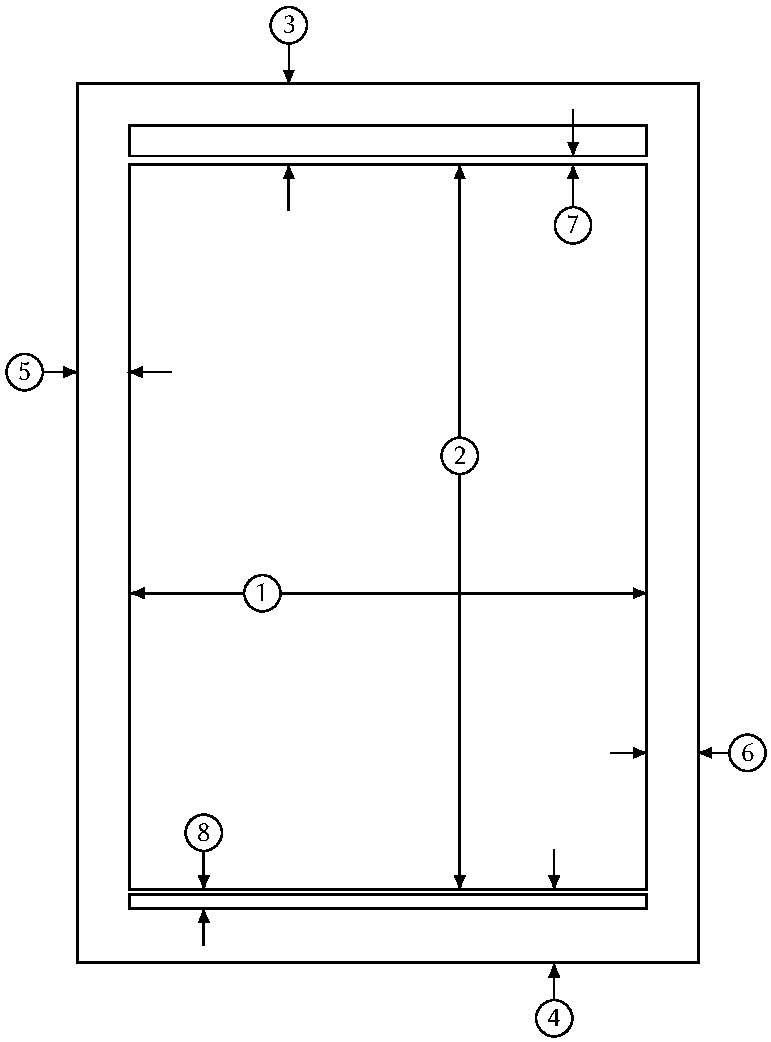
\includegraphics[width=\columnwidth]{figures/page-layout}
%   \caption{\emph{Layout} da página. O tamanho é A4 (210\,x\,297\,mm);
%     a mancha de texto (1 e 2) mede 175\,x\,246\,mm; a margem superior
%     (3) é 26\,mm e a margem inferior (4) é 23\,mm; as margens esquerda
%     (5) e direita (6) medem 17,5\,mm; o espaço entre o cabeçalho e o
%     texto (7) é 10\,pt; a distância entre o final do texto e o final do
%     rodapé (8) é 18\,pt; o espaço entre as colunas (não mostrado) é
%     18\,pt.\label{fig:page-layout}}
% \end{figure}

% \section{Cabeçalho}

% O cabeçalho do artigo tem duas variações, uma para a primeira página e outra para as páginas seguintes. Ambas são descritas nas subseções a seguir.

% \subsection{Cabeçalho da Primeira Página}

% Na primeira página, o cabeçalho apresenta o título da série e o ano da edição em uma primeira linha. A segunda linha traz a descrição da licença de publicação, que para os eventos que disponibilizam seus artigos na SBC OpenLib corresponde à licença CC BY-NC 4.0. Os autores devem preencher a informação do título da série, acrônimo do evento e ano do evento nos campos \textit{jtitle}, \textit{jid} e \textit{jyear}, respectivamente. A informação sobre a licença deve constar do campo \textit{copyrightstatement}.

% \subsection{Cabeçalho da Página 2 em diante}

% A partir da página 2, o cabeçalho apresenta o título resumido à esquerda e a lista de autores resumida à direita. O título abreviado do artigo e a lista abreviada de autores devem ser preenchidos em \textit{shorttitle} e \textit{shortauthors}, respectivamente.

% \section{Abertura}

% O preâmbulo do artigo contém os principais metadados que descrevem o artigo: o título, o resumo e as palavras-chave, tanto em inglês, quanto em português.

% \subsection{Título}

% \subsection{Autores}

% \section{Bibliografia}

% Citações e referências bibliográficas devem seguir o formato definido pela ABNT (NBR\,10520, versão 2002 e NBR\,6023 versão 2002 ou, preferencialmente, 2018). Os organizadores de cada evento definem se as citações seguirão o formato numérico ou autor-data. Observe que:

% \begin{itemize}
%   \item Endereços web (URLs) não são colocados entre ``<\,>'' (esse é o padrão na versão 2018 da NBR\,6023)
%   \item ``In'' e ``et al.'' são formatados em itálico (esse é o padrão na versão 2018 da NBR\,6023)
%   \item No formato numérico, os sobrenomes não são grafados em caixa alta
%   \item No formato autor-data, usa-se versalete para os sobrenomes (com a primeira letra maiúscula)
% \end{itemize}

% \section{Outros exemplos}

% Esta classe é baseada na classe \texttt{article} e, portanto, os comandos usuais de \LaTeX, como \textsf{\textbackslash{}verse}, \textsf{\textbackslash{}quotation} etc. podem ser usados normalmente:

% \begin{verse}
%   Batatinha quando nasce\\
%   Espalha a rama pelo chão

%   A menina quando dorme\\
%   Põe a mão no coração
% \end{verse}

% \begin{quotation}
%   \itshape
%   Algum tempo hesitei se devia abrir estas memórias pelo princípio ou
%   pelo fim, isto é, se poria em primeiro lugar o meu nascimento ou a
%   minha morte. Suposto o uso vulgar seja começar pelo nascimento,
%   duas considerações me levaram a adotar diferente método: a
%   primeira é que eu não sou propriamente um autor defunto, mas um
%   defunto autor, para quem a campa foi outro berço; a segunda é que
%   o escrito ficaria assim mais galante e mais novo. Moisés, que também
%   contou a sua morte, não a pôs no intróito, mas no cabo: diferença
%   radical entre este livro e o Pentateuco.
% \end{quotation}

% Equações de segundo grau (Equação \ref{eq:2grau}) são estudadas no ensino
% médio. As raízes de uma equação de segundo grau podem ser encontradas
% por~\eqref{eq:bhaskara} --- a fórmula de Bháskara. O valor do discriminante
% $\Delta$ (Equação \ref{eq:delta}) determina se a equação tem zero, uma ou
% duas raízes reais distintas.

% \begin{equation}
%   \label{eq:2grau}
%   ax^2+bx+c=y \quad \forall x \in \mathbb{R}
% \end{equation}

% \begin{gather}
%   \label{eq:bhaskara}
%   y=0 \Leftrightarrow x=\frac{-b \pm \sqrt{\Delta}}{2a}
%   \Leftrightarrow x \text{ é raiz da equação}\\
%   \label{eq:delta}
%   \Delta\enspace(\mathit{delta}) = b^2-4ac
% \end{gather}

% \begin{figure}
%   \centering
%   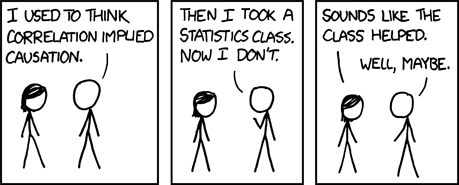
\includegraphics[width=\columnwidth]{figures/xkcd_552_correlation}
%   \caption{A bitmap figure (from \url{xkcd.com/552}).\label{fig:xkcd-correlation}}
% \end{figure}

% \begin{figure*}[b]
%   \centering
%   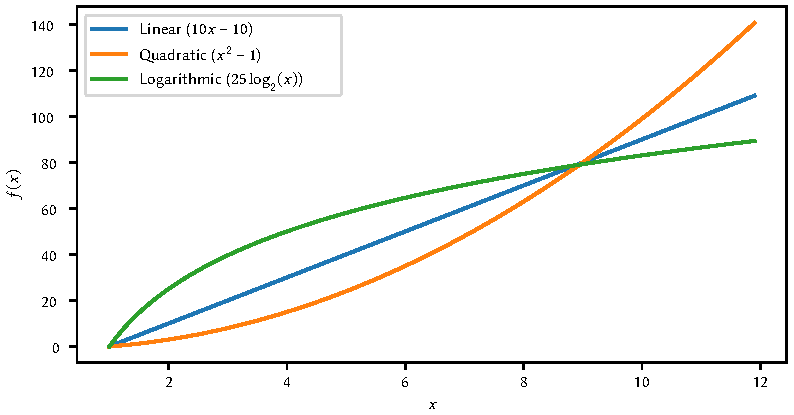
\includegraphics{figures/graph-functions}
%   \caption{A vector figure spanning both text columns.\label{fig:graph-functions}}
% \end{figure*}

% Imagens vetoriais (como diagramas e gráficos, a exemplo das Figuras~\ref{fig:page-layout}~e~\ref{fig:graph-functions}) \emph{não} devem ser convertidas para \emph{bitmaps}, mas sim mantidas em algum formato vetorial, como PDF. Imagens não-vetoriais com cores predominantemente sólidas (como a Figura~\ref{fig:xkcd-correlation}) devem ser convertidas para o formato PNG e imagens fotográficas ou com texturas devem ser convertidas para o formato JPEG. Uma figura ou tabela muito grande (Figura~\ref{fig:graph-functions}, Tabela~\ref{tab:form}) pode excepcionalmente ocupar a largura das duas colunas de texto, mas apenas no início ou no final da página. Todas as figuras e tabelas devem ser acompanhadas das respectivas legendas explicativas numeradas logo abaixo delas.

% \begin{table*}
%   \centering
%   \newcolumntype{M}[1]{>{\centering}m{#1\textwidth}}
%   \begin{threeparttable}
%     \begin{tabular}{|M{0.265}|M{0.073}|M{0.084}|M{0.073}|M{0.073}|M{0.08}|M{0.082}|M{0.067}|}
%       \hline
%       \textbf{Experimento número:} & \multicolumn{2}{c|}{1}                         & \multicolumn{4}{c|}{\textbf{Data:}} & jan 2017
%       \tabularnewline \hline
%       \textbf{Título:}             & \multicolumn{7}{c|}{Medições iniciais}
%       \tabularnewline \hline
%       \textbf{Tipo:}               & \multicolumn{7}{c|}{Levantamento quantitativo}
%       \tabularnewline \hline \hline
%       \textbf{Locais}              & São Paulo                                      & Rio de Janeiro                      & Porto Alegre & Recife & Manaus & Brasília & Rio Branco
%       \tabularnewline \hline
%       \textbf{Valores obtidos}     & 0.2                                            & 0.3                                 & 0.2          & 0.7    & 0.5    & 0.1      & 0.4\tnote{a}
%       \tabularnewline \hline
%     \end{tabular}
%     \begin{tablenotes}
%       \item[a] This is an example of table footnote with a reference
%       \item This is an example of table footnote without a reference
%     \end{tablenotes}
%     \caption{A table spanning both text columns.\label{tab:form}}
%   \end{threeparttable}
% \end{table*}

% \section{Conclusion}

% \begin{itemize}
%   \item @Book: \cite{Knuth:96}.

%   \item @Article (em periódico): \cite{floats2014}.

%   \item @InProceedings (ou @Conference): \cite{alves03:simi}.

%   \item @InCollection (capítulo de livro ou coletânea): \cite{bobaoglu93:concepts}.

%   \item @PhdThesis: \cite{garcia01:PhD}.

%   \item @MastersThesis: \cite{schmidt03:MSc}.

%   \item @Techreport: \cite{alvisi99:analysisCIC}.

%   \item @Manual: \cite{biblatex}.

%   \item @Misc: \cite{gridftp}.

%   \item @Online (para referência a artigo \emph{online}): \cite{fowler04:designDead}.

%   \item @Online (para referência a página web): \cite{FSF:GNU-GPL}.

%   \item @article (para referência a página web): \cite{alon09:how}.

% \end{itemize}


\end{document}
